\documentclass[10pt,twoside,twocolumn,openany]{book}
\usepackage[bg-letter]{dnd} % Options: bg-a4, bg-letter, bg-full, bg-print, bg-none.
\usepackage[english]{babel}
\usepackage[utf8]{inputenc}
\usepackage{graphicx}

% Start document
\begin{document}
\fontfamily{ppl}\selectfont % Set text font

\chapter{Hyrule Races}

% Goron race
\section{Goron}

\subsection{Physiology}
Gorons stand taller and wider than hylians, and universally have skin of an orange-brown hue. What little "hair" they possess is so stiff and thick it resembles solid rock, and usually grows only high on a goron's scalp and across its upper back. A few gorons are also able to grow beards or other facial hair, especially if they are of advanced age. A pair of goron eyes are wide set, perfectly circular, and completely dark—posessing no whites like those of a hylian's or gerudo's eyes. Goron noses are flat. Jaws are very wide, powerful, and composed entirely of molars—used to crush and pulverize the rocks which famously make up goron diets.\\
Although they are physiologically more similar to earth elementals than mammals, gorons nonetheless take a humanoid shape. They are required to eat and sleep to live. Drinking serves no purpose for them. They can persist indefinitely without breathing, but doing so is unpleasant, especially when the goron is exerting itself. Mysteriously, gorons dine on rocks and other solid minerals—tastes vary between tribes, as some prefer coarse ores, others savor gemstones, but they generally dislike less solid earth such as sand or dirt. A few dine on more traditional foods such as meat or mushrooms, but this seems to be for pleasure rather than sustenance.\\
Because they are literally made of rock, gorons have an inherent durability to their bodies, but are also particularly dense and heavy. This makes traditional movement difficult for them over anything but short distances. When traveling more than a few feet, a goron will usually tuck itself into a ball and roll, which allows it to traverse ground at much greater speed. This speed of this "goron roll" combined with a goron's weight makes it a powerful charging attack for chasing down foes. Aside from this, gorons battle with powerful punches—punches so powerful that fighting unarmed is the norm among their race.\\
Gorons only possess one apparent sex, which they universally refer to as male. "Brother" is a very common term of endearment among them, and friends of a goron tribe are often referred to as brothers—regardless of whether or not they are male.

\subsection{Society}
Goron cities and villages are almost universally built into caves or the sides of mountains, where the tastiest and most nutritious rocks are abundant. Their reliance on 
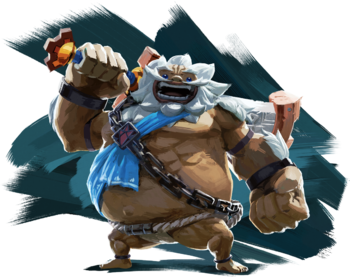
\includegraphics[width=100mm,scale=0.5]{daruk.png} \\
eating rocks makes their cultures particularly dependent on mining to survive, to the extent that the majority of gorons have experience in this profession. Many anthropologists believe gorons evolved to be as physically powerful and enduring as they are due to their race's inherent dependency on mining. Stronger gorons with greater strength made better miners, which enabled them to better survive and provide for their kin.\\
Due to their mining dependency, goron culture heavily involves stonework and the working of metals. Blacksmiths are abundant among them, and their structures are constructed almost entirely of metal. They're also one of few races that has widely adapted the use of blackpowder, and when in battle they often make use of bombs or other explosives. Their resistance to heat gives them an edge over most foes when using such powerful, but esoteric weapons.\\
Gorons almost always place a high degree of value on physical strength and stamina, pride, honesty, and trustworthiness. Gorons most readily get along with races which share these values, usually including the like of subrosians, rito, and most hylians. A friend is rarely lost on a goron unless that friend is caught in a lie. Unsurprisingly, gorons often have a difficult time with people from less prideful cultures.

\subsection{Goron Names}
Goron names are all considered male. These names more often than not consist of at least one "go" or "da" syllable. Deep vowel sounds such as "ah," "oh," and "oo" are prominent. "R" consonants are also very common, especially in the center of the name. \\
\textbf{Male:} Biggoron, Darbus, Daruk, Darmani, Darunia, Gongoron, Gorko, Gortram, Kabetta, Kagoron, Medigoron, Reagah, Rohan, Tanko, Volcon, Yunobo. 

\subsection{Goron Traits}
Built like mountains, eating rocks, and wading through lava — gorons are nothing if not hardy and impregnable.
\indent \textbf{Ability Score Increase.} Your Strength score increases by 2 and your Constitution scores increases by 1.\\
\indent \textbf{Age.} Gorons reach adulthood in about a decade, but can live to be over a century. \\
\indent \textbf{Alignment.} Although gorons can alienate those outside their kin group, they form strong bonds with those they trust. They have a tendency towards lawful good.\\
\indent \textbf{Size.} Gorons are usually between 6 and 8 feet in height, and quite stocky. Your size is Medium.\\
\indent \textbf{Speed.} Your base walking speed is 25 feet.\\
\indent \textbf{Hot Skin.} You have advantage on saving throws against fire damage, resistance to fire damage, and are unable to catch flame. On the other hand, you have disadvantage on all saving throws against cold damage.\\
\indent \textbf{Stone Armor.} Your skin is hard as stone. When you aren’t wearing armor and not wielding a shield, your AC is 13 + your Constitution modifier.\\
\indent \textbf{Darkvision.} Accustomed to life underground, you have superior vision in dark and dim conditions. You can see in dim light within 60 feet of you as if it were bright light, and in darkness as if it were dim light. You can’t discern color in darkness, only shades of gray.\\
\indent \textbf{Natural Athlete.} You are proficient in the Athletics skill.\\
\indent \textbf{Like Stone.} You can attempt to hide when you are surrounded by any kind of rocky terrain. Additionally, you can move across difficult terrain made of earth or stone without expending extra movement.\\
\indent \textbf{Stone in the Water.} You sink to the bottom of any body of water you enter. Also, you have no need to drink water, and can hold your breath indefinitely. While underwater, you have disadvantage on all ability checks and attack rolls.\\
\indent \textbf{Goron Roll.} When you take the Dash action, you gain the extra movement you otherwise would plus 20. If you take the Dash action and move at least 20 feet straight towards a creature, you can make a roll attack against that creature as a bonus action. This attack counts as an unarmed strike against the target and its damage is decided by a d4 dice roll plus your Strength modifier. This dice changes as you level up, as shown in the Roll Attack table. 
\begin{dndtable}
 	\textbf{Goron Level}  & \textbf{Roll Attack Damage} \\
    1st  & 1d4 + Strength Modifier \\
 	5th  & 1d6 + Strength Modifier\\
  	11th  & 1d8 + Strength Modifier\\
    17th  & 1d10 + Strength Modifier\\
\end{dndtable}
\indent \textbf{Rock Gourmet.} You are able to eat half a pound of rock instead of consuming a portion of rations whenever you feel hungry.\\
\indent \textbf{Languages.} You can speak, read, and write Common and Goro.

% Zora race
\newpage
\section{Zora}

\subsection{Physiology}

Amphibious, fish-like humanoids, zora have sleek and glistening bodies. Zora rarely breed, but when they do, they have offspring in batches of eggs ranging from 1 to 8, which grow into tadpoles, and eventually amphibious humanoids. Zora age at a slow rate compared to hylians, but have a growth spurt and reach adulthood around the age of 20, reach middle age at about 100 years, and can occasionally live to be more than 200.
The exact shape and demeanor of zora is heavily dependent on the two subraces: sea zora, and river zora. "Sea zora" have evolved to live in deeper saltwater, and "river zora" have evolved to live in shallower freshwater, but modern zora of either variety can be found in either habitat.\\
Sea zora are taller and more slender, and have a pale white chest and face, with a backside of a darker color—usually blue, but occasionally red, gray, brown, or other colors. The shape of a sea zora's head varies widely, but usually has a backside resembling some variety of fish tail, with fins that further aid its ability to swim.\\

\subsection{Society}

Due to their amphibious nature, zora villages are most often built along coastlines, rivers, lakes, and other areas that blend shallow water with nearby land. This enables them to effectively evade and defend against predators that are exclusive to land or sea, and hunt more effectively from both sources. Zora usually wear a small amount of jewelry or armor, but less clothing than races such as hylians or rito, as excess clothing hampers their ability to swim.\\
A given zora tribe is usually ruled by a royal family of zora, to which the tribe is loyal for generations. The current monarch of a tribe is often referred to with a title such as "King Zora" or "Queen Zora" than his or her actual name.\\
Royal families are usually allies with the royal families of hylians. They frequently intermingle with other races who live on coastlines, and are renowned for their unique style of music.

\subsection{Zora Names}

\textbf{Male:} Cleff, Japas, Mikau, Ralis, Sidon, Tijo, Toto \\
\textbf{Female:} Laruto, Lulu, Mipha, Oren, Rutela, Ruto 

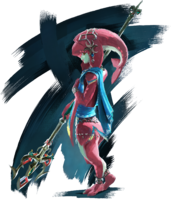
\includegraphics[width=65mm,scale=0.5]{mipha.png} \\

\subsection{Zora Traits}
Zora claim the title of the only truly amphibious race in Hyrule — and are the second most populous, exceeded only by hylians.\\
\indent \textbf{Ability Score Increase.} Your Wisdom score increases by 2 and your Dexterity score increases by 1.\\
\indent \textbf{Age.} Zora reach adulthood by the age of 20 at the earliest, and can live to an age of 200 or more.\\
\indent \textbf{Alignment.} Zora tend towards lawful neutral.\\
\indent \textbf{Size.} A zora can vary greatly in size, but is usually about 6 feet tall. Rarely, a zora can grow to a height of 8 feet or more. Your size is Medium.\\
\indent \textbf{Speed.} Your base walking speed is 30 feet, and you have a swim speed of 60 feet.\\
\indent \textbf{Amphibious.} You can breathe both air and water.\\
\indent \textbf{Underwater Camouflage.} When you make a Dexterity (Stealth) check while mostly or entirely underwater, you do so with advantage. \\
\indent \textbf{One with the Water.} You have advantage on all Acrobatics, Animal Handling, Nature and Survival ability checks that involve water or any animal that lives in a wet environment.\\
\indent \textbf{Fire Vulnerability.} You are vulnerable to fire damage attacks.\\
\indent \textbf{Keen Senses.} You have proficiency in the Perception skill.\\
\indent \textbf{Lightning Field.} You can cast the lightning field cantrip. Wisdom is your casting ability for this spell. \\
\indent \textbf{Ancestral Arms.} You have proficiency with the arm blade, pike, net, spear, and trident. If you otherwise gain proficiency with spears or tridents, you gain a +1 bonus on damage rolls with these weapons.\\
\indent \textbf{Languages.} You can speak, write, and read Common and Zoran.
\newpage
% Korok race

\section{Korok}

\subsection{History}

According to legend, koroks were originally created many eons ago by the Great Deku Tree to spread plant life across the entire world. This legend portends that every tree which still grows can trace its ancestry back to a seed planted by a korok. Regardless of whether or not this is true, modern koroks are clearly magical creatures not directly related to any other races, and they retain an unusually profound understanding of the natural world.\\
Despite the innate curiosity of koroks, they are dissuaded by the Deku Tree from leaving the forest unless they have an important reason to do so. Indeed, the world outside the woods is dangerous to a typical korok. In the modern world, few people who dwell outside of forests know much of this race. They are so rare, so bizarre, and so elusive that they are frequently delegated to myth.

\subsection{Physiology}

A typical korok stands between 2 and 3 feet, with an oblong body composed of hollow wood, and particularly short limbs. Indeed, koroks are extremely lightweight and buoyant.\\
A korok's face is most unusual. If left unadorned, a korok face is comprised only of a nose-like stick protruding outward. Almost every korok will instead construct a mask to serve as its apparent face. This mask almost always is comprised of a large leaf with holes cut into it—one hole to anchor the mask on its "nose," two holes to serve as "eyes," and finally one to serve as a "mouth." Koroks seemingly have no physical need to construct these masks, but it is done in part so they can express their personality and in part so koroks can better recognize each other. Koroks tend to be very fascinated by creatures who are naturally more expressive than themselves, and it seems these masks are modeled after such creatures.\\
Although koroks can be created by the Deku Tree's magic, they can also reproduce on their own, unlike kokiri. A korok can produce more koroks simply by planting seeds and caring for them until they grow to maturity, although this is a relatively rare practice performed only a few times in a korok's long lifespan. Despite technically being parent and child, these two koroks would consider themselves more akin to an older sibling and a younger one.\\
A korok reaches its full size less than two years after being planted, and usually gains mobility a long time before that. The earliest a korok can produce a seed of its own seems to be about 2 or 3 years, but it will often live for decades before it decides to do so.\\
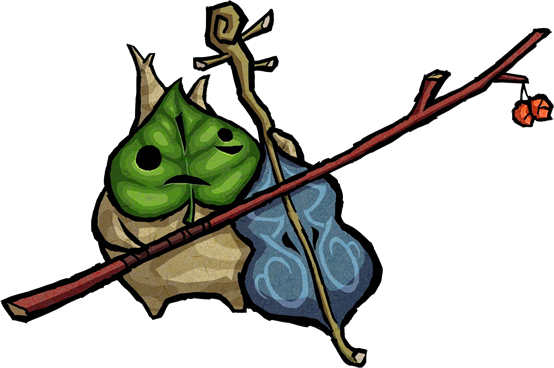
\includegraphics[width=100mm,scale=0.5]{makar.png} \\
As they don't produce sexually, koroks don't have traditional genders. They don't truly consider themselves male, unlike the all-male goron race, but usually default to male pronouns anyway.

\subsection{Society}

Koroks tend to be very optimistic, curious, altruistic, excitable, energetic, and playful.\\
They predominantly live in forests protected by the Great Deku Tree, often among kokiri, and usually only leave these woodlands temporarily. Much like kokiri, they are considered the "children" of the Deku Tree. They are much more widespread than kokiri, however, likely due to the fact they can reproduce on their own.\\
A korok's needs and therefore its responsibilities are simple. It doesn't require food, can fly or hide from most herbivores, can sleep almost anywhere, and doesn't need to care for its young nor bother much with reproduction. A korok is nonetheless restless and eager to do something—anything. Thus, a typical korok often occupies much of its time playing elaborate games, or exploring the vast wilderness of Hyrule. Many pursue a self-learned art, profession, or expertise—something it can master over the many years it lives. When the Deku Tree has a job that needs doing, there's always at least one korok eager to do it.\\
Perhaps because of this energetic nature, the surprisingly few times koroks interact with races outside the forest, they are nothing but helpful. Many a legend has been told of these altruistic but secretive creatures—completing chores will hylians sleep, saving children from wells, and so on.\\

\subsection{Korok Names}

Korok names tend to be rather short, rarely comprised of more than two brief syllables.\\
\textbf{Examples:} Aldo, Chio, Daz, Drona, Elma, Hestu, Hollo, Irch, Kula, Linder, Maca, Makar, Oakin, Olivio, Pepp, Peeks, Natie, Rown, Walton 

\subsection{Korok Traits}

Small, peaceful, immortal, and child-like plant creatures. They aren't much for combat or stealth, but it's hard not to smile around them.\\
\indent \textbf{Ability Score Increase.} Both your Charisma and Dexterity scores increase by 2.\\
\indent \textbf{Age.}Age. A korok reaches physical maturity after less than 2 years, but can live for up to 200 years or more. It retains a childlike innocence throughout its entire life.\\
\indent \textbf{Alignment.} Koroks strive to populate the world with trees, preserve life, and are eagerly help anyone who needs it. They have an extreme tendency towards all forms of good.\\
\indent \textbf{Size.} A typical korok’s height averages about 3 feet. Your size is Small.\\
\indent \textbf{Speed.} Your base walking speed is 25 feet.\\
\indent \textbf{Type.} You are considered both a humanoid and a plant for any effect relating to your type.\\
\indent \textbf{Natural Cantrip.} You know the druidcraft cantrip.\\
\indent \textbf{Jingle.} Your body produces an unusual jingling noise whenever you move, which grows louder the more violently you move. You have disadvantage on Dexterity (Stealth) checks to move quietly.\\
\indent \textbf{Fire Vulnerability.} You are vulnerable to all sorts of fire damage. \\
\indent \textbf{Korok Copter.} As an action, you can grow from your wrist a magical plant that is as tall as your body, and adorned with a pair of spinning wings. You can control the wings of this plant in such a way that you effectively gain a flying speed of 25 feet. Maintaining flight requires dedication from this hand, preventing that hand from being used for anything else, but otherwise maintaining flight or hovering in place is effortless for you. You can detach the magical plant as an action or bonus action, which causes it to wither away into ash almost instantly. Until you dismiss the plant, it is considered part of your body, and any damage dealt to it is dealt to you.\\
\indent \textbf{Natural Performer.} You are proficient in both the Performance and the Nature skills. Additionally, you can survive without food, so long as you have water, sunlight, and air.\\
\indent \textbf{Ancient Knowledge.} You gain proficiency in one of the following skills: Arcana, History, Medicine, Performance, or Religion. Alternatively, you can gain proficiency in any one tool.\\
\indent \textbf{Tool Proficiency.} Most koroks adapt to a particular profession. You gain proficiency in one artisan's tool or one musical instrument of your choice.\\
\indent \textbf{Nature's Guise.} You can attempt to hide when surrounded by any area that is filled with trees or even when you are only lightly obscured by foliage, heavy rain, falling snow, mist, and other natural phenomena.\\
\indent \textbf{Languages.} You can speak, write and read both Common and Deku.

% Spells from the world of Hyrule
\chapter{Hyrule Spells}
%The spells are presented in alphabetical order.

\section{Lightning Field}
\textit{Evocation Cantrip} \\

\noindent \textbf{Casting Time:} 1 action\\
\textbf{Range:} 5 feet\\
\textbf{Components:} S\\
\textbf{Duration:} Instantaneous\\

\noindent A cylindrical aura of electricity sweeps around you for a moment, jolting adjacent foes. Each creature within range, other than you, must succeed on a Dexterity saving throw or take 1d6 lightning damage. \\
This spell's damage increases by 1d6 when you reach 5th level (2d6), 11th level (3d6), and 17th level (4d6). \\

%\begin{commentbox}{Neat Green Box!}
%	\lipsum[1]
%\end{commentbox}

%\subtitlesection{Weapon, +1, +2, or +3}
%{Weapon (any), uncommon (+1), rare (+2), or very rare (+3)}

%\begin{quotebox}
%	As you approach this template you get a sense that the blood and tears of many generations went into its making. A warm feeling welcomes you as you type your first words.
%\end{quotebox}

%\newpage % Acts as columbreak because of twocolumn option; for pagebreak use \clearpage

% For more columns, you can say \begin{dndtable}[your options here}.
% For instance, if you wanted three columns, you could say
% \begin{dndtable}{XXX}. The usual host of tabular parameters are
% aailable as well.
%\header{Nice table}


%\begin{paperbox}{Do the Players need direction?}
%	\lipsum[1]
%\end{paperbox}

% You can optionally not include the background by saying
% begin{monsterboxnobg}
\begin{comment}
\begin{monsterbox}{Monster Foo}
	\textit{Small metasyntactic variable (goblinoid), neutral evil}\\
	\hline
	\basics[%
	armorclass = 12,
	hitpoints  = 16 (3d8 + 3),
	speed      = 50 ft
	]
	\hline
	\stats[
    STR = \stat{12}, % This stat command will autocomplete the modifier for you
    DEX = \stat{7}
	]
	\hline
	\details[%
	% If you want to use commas in these sections, enclose the
	% description in braces.
	% I'm so sorry.
	languages = {Common Lisp, Erlang},
	]
	\hline \\[1mm]
	\begin{monsteraction}[Monster-super-powers]
		This Monster has some serious superpowers!
	\end{monsteraction}
	\monstersection{Actions}
	\begin{monsteraction}[Generate text]
		This one can generate tremendous amounts of text! Though only when it wants to.
	\end{monsteraction}

	\begin{monsteraction}[More actions]
    See, here he goes again! Yet more text.
	\end{monsteraction}
\end{monsterbox}
\end{comment}
% End document
\end{document}
